\documentclass[a4paper, 11pt]{article}
\usepackage[english]{babel}  
\usepackage[utf8]{inputenc} 
\usepackage[centertags]{amsmath}
\usepackage{amssymb,amsfonts,amsthm}
\usepackage{indentfirst}
\usepackage{array}
\usepackage{float}
\usepackage[usenames,dvipsnames,svgnames,table]{xcolor}
\usepackage{hyperref}
\usepackage{enumerate}
\usepackage{graphicx}
\usepackage{epstopdf}
\usepackage{graphics}
\usepackage{subfigure}
\usepackage[margin=1in]{geometry} 
\usepackage{listings}
\usepackage{setspace}
\usepackage{multirow}
\usepackage{graphicx}
\usepackage{comment}

\begin{document}

	\begin{center}
		\sc\large\textbf{Personalized Apartment Recommender}\\
			\noindent {\small  TEAM 153:
        	Ansel Lim,
        	Daosheng Lin
        	Hong Wen (Key) Tai,
        	Keith Loo}
	\end{center}

{All team members contributed equally to the project. Ansel performed data collection and scoring and edited the report and poster. Daosheng designed the user preferences questionnaire, performed the experiments, and wrote the report and poster. Key designed the scoring algorithm and worked on database design and data retrieval. Keith worked on data visualization and the map's user interface. Everyone participated in literature review, code review and review of this manuscript.}

	\section{Introduction: Motivation \& Problem Definition}
	
	Home buyers in Singapore typically obtain their information from (a) social media (e.g. blogs, Instagram, YouTube, forums), (b) browsing commercial real estate websites (e.g. PropertyGuru, 99.co), (c) online advertisements, (d) messaging applications (e.g. WhatsApp, Telegram), (e) old media (e.g. newspapers, television) and (f) word of mouth. Multiple sources of information may lead to confusing and conflicting conclusions. Furthermore, as alluded to by Kavey (1989) [4], the search for homes may be constrained by the bias present in the information provided by realtors.
	
	Home buyers also want competitively priced homes. B.H. Chua (2015) [1] and C. Y. Yiu \& C. M. Hui (2005) [2] discussed the problems of persistent increases in property prices in Singapore. Accurate information is key to formulating timing strategies, which are very important in real estate investments, as discussed by Teck Chin \& Geofrey Mills (1999) [3].

 Aspiring homebuyers in Singapore need an informative toopl to analyze and visualize unbiased open-source information, and generate personalized, affordable recommendations based on their preferences and constraints.

	\section{Methodology}
	
	\subsection{Intuition}
	
	Most tools for researching the property market involve filtering for property-specific attributes, such as location, price and size of the apartment. However, the thought process that goes into purchasing a home involves a much greater variety of factors \textit{beyond} attributes of the property, such as proximity to various amenities (e.g. restaurants, schools, and recreational facilities). Depending on demographic factors and stage of life, individuals may have different priorities and preferences as to neighborhood amenities, which do play a role in property search.
	
	The market needs a property recommendation tool which incorporates the rich information available in neighborhood amenities, enabling personalized, visualizable recommendations.
	
	\subsection{Data collection and preprocessing}
	
	The Government of Singapore maintains and publishes publicly available datasets (e.g. www.data.gov.sg), and OneMap API, a map API. Through these sources, we were downloaded and scraped details of residential projects (e.g. past sale transactions, addresses, map coordinates) and locations of various amenities (e.g. parks, educational institutions, food and beverage establishments). We further enriched the information with data from Google Places API, adding details such as review ratings and number of reviews. 
	
	The raw data was stored in multiple comma separated values (CSV) files, and subsequently formatted into a consistent schema and loaded into an SQLite database. The data was stored in two tables, (1) a “properties” table, containing details of the various residential housing projects such as name, district, location, average transacted price, and (2) a “features” table, containing details of the different amenities such as name, category, location, and review ratings. In total, we retrieved 10,614 rows of property transaction data and 32,695 rows of amenities data over 15 different types of amenities (subsidized clinics, community centers, gyms, hawker centers, shopping malls, public sports facilities, parks, primary schools, secondary schools, supermarkets, food and beverage establishments, bus stops, carparks, subway stations, and taxi stands).
	
	\begin{comment}
	Number of properties is 11,488 if Batch 4 is fixed.
	\end{comment}

    \subsection{User preferences questionnaire}
    
    The landing page of our tool is a user preferences questionnaire which was designed with the Flask web framework. This consists of a mix of “hard constraints” and “preferences”. Hard constraints refer to price per square meter, district, and apartment type (public housing or condominiums). Preferences refer to a ranking of the importance of each attribute. For example, young parents may prefer homes close to good schools. The user's constraints and preferences are stored and passed to the scoring system.
    
   \begin{figure}[h]
   \centering
   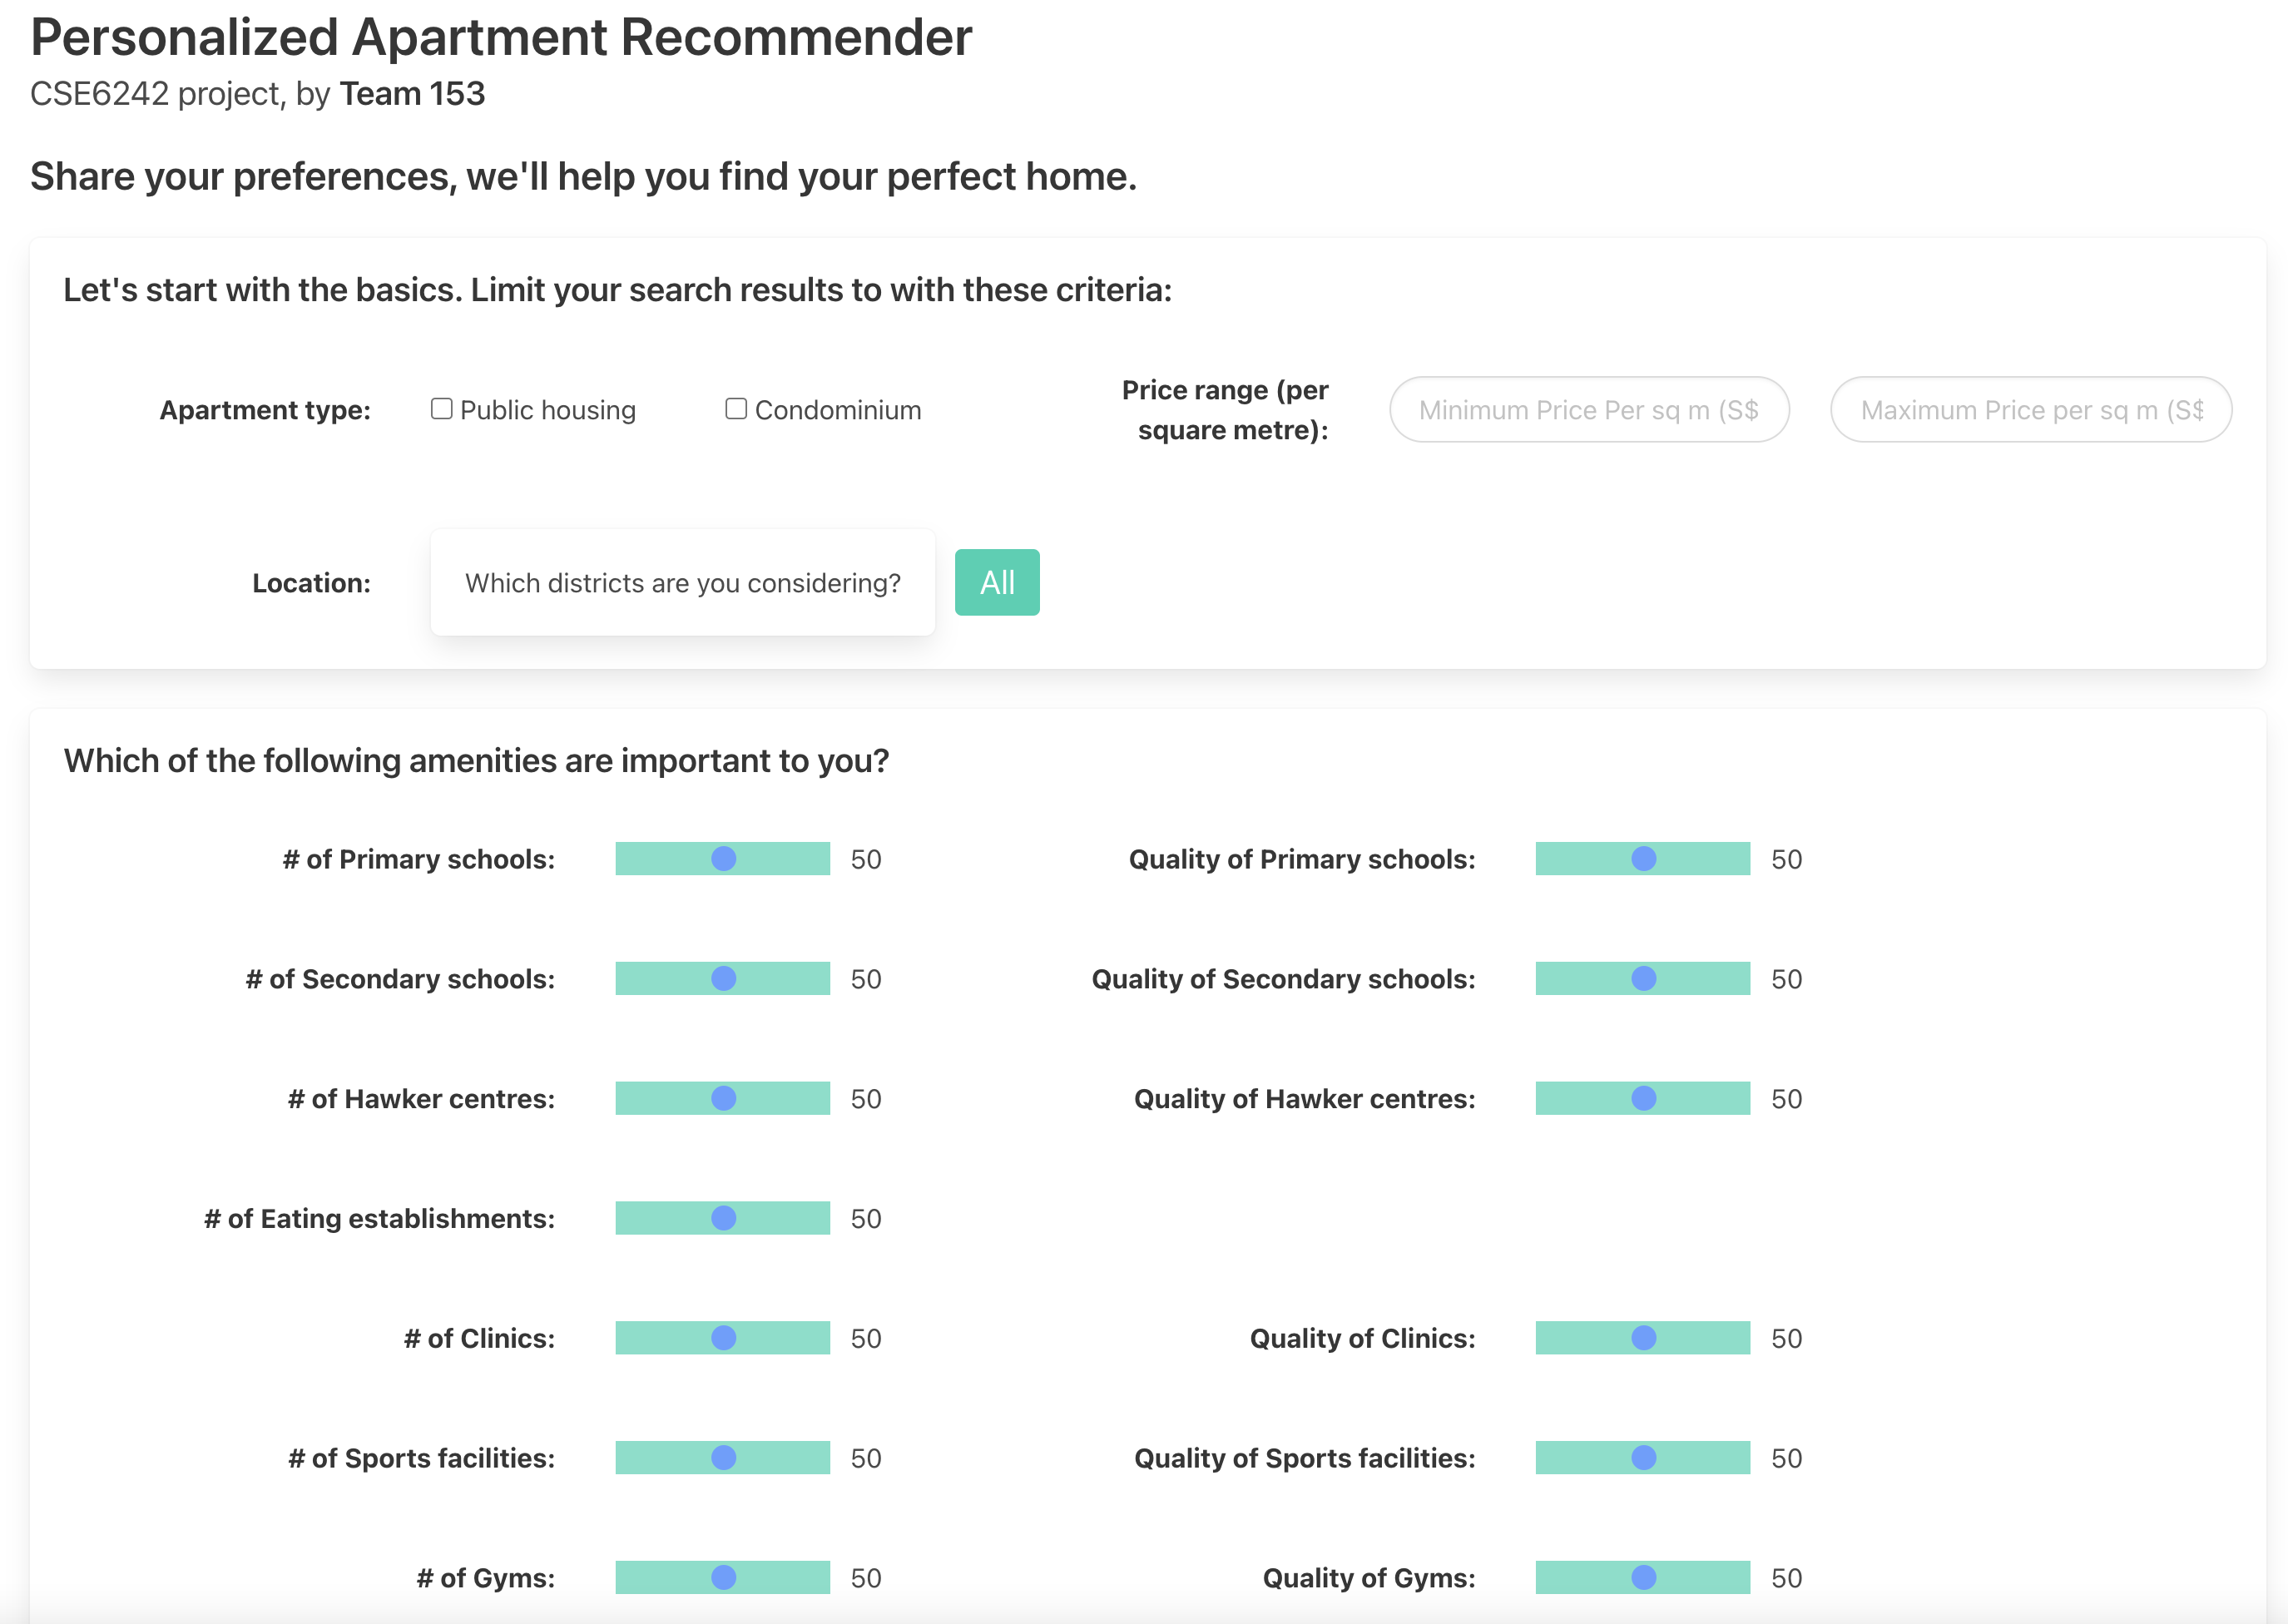
\includegraphics[width={0.5\textwidth}]{questionnaire.png}
   \caption{Part of the user preferences questionnaire}
   \end{figure}
    
    \subsection{Review of scoring methodology in recommendation systems} 
    Various insightful methods in decision science exist in the literature. B. Song \& S. Kang (2015) [5] propose assignment of “weights” to different user inputs and attributes according to user-specified rankings, which we may adopt. However, this is not a dynamic solution; the process of arriving at the calculated weights is not ideal in a web application as it is difficult to keep users engaged during the intervening computation time. M. Morita \& Y. Shinoda (1994) [6] explore user reading times as a gauge of the relevancy of search results. This concept of using user engagement attributes may be explored in the design of our scoring algorithm. S. Opricovic \& G.H. Tzeng (2002) [7] discuss the use of two multiple-criteria decision-making methods, VIKOR and TOPSIS, in finding optimal solutions, however this may not be computationally feasible in large-scale evaluation of hundreds or thousands of alternative results. 
    
    Isinkaye, F. O., Folajimi, Y. O., \& Ojokoh, B. A. (2015) [8] discuss different techniques used in real estate recommender systems such as content-based and collaborative filtering methods. Deldjoo, Y., Dacrema, M.F., Constantin, M.G., et al. (2019) [9] explore a novel hybrid method which not only performs better than a pure content-based filtering method, but is also able to deal with the “cold start problem”. However, the paper had existing user-item interaction data which is not available to us from publicly available data sources. Therefore, we will have to use a pure content-based approach that relies on item features. 
    
    Interestingly, Lops, P., Jannach, D., Musto, C. et al. (2019) [10] share about developments for content-based recommendations such as enriching features using multimedia data or using embeddings to encode item features. We can possibly explore using such methods to improve our recommendations. 
    
    Computing similarity between houses can be a very computationally intensive process. J. Leskovec, A. Rajaraman, \& J. D. Ullman (2014) [11] discuss several methods of finding similar items efficiently, such as using cosine distance to compare similarity between items and using locality-sensitive hashing to hash similar items into buckets. This effectively reduces the search space to items which have the same bucket. By confining our search space to houses within the same hash bucket, we may recommend homes more efficiently. 

    \subsection{Our scoring methodology}
    
\subsubsection{General method of scoring}    
    
    Putting our research into application, our scoring method takes into account input weights from the user, as well as attribute scores for each housing project. Both the input weights and attribute scores have a range of 0 to 1, and the overall score will be the weighted sum of scores. As an illustrative example, assume that there are only two attributes (schools and public transport). The user places less importance on schools and gives a weight of  0.3 ($w_{\text{school}}  = 0.3$), and values the public transport links in the area thus assigns a weight of 0.8 to public transport ($w_{\text{transport}}  = 0.8$). Each housing project has a pre-computed score for each attribute; housing project A can have 0.8 as its score for schools ($s_{A,\text{school}} = 0.8$) and 0.5 as its score for public transport ($s_{A,\text{transport}} = 0.5$), whereas housing project B can have 0.4 as its score for schools ($s_{B,\text{school}} = 0.4$) and 0.9 as its score for public transport ($s_{B,\text{transport}} = 0.9$). Using the above examples, the overall score of housing project A will be:
    
\[ w_{\text{school}} \times s_{A,\text{school}} + w_{\text{transport}} \times s_{A,\text{transport}} = 0.3 \times 0.8 + 0.8 \times 0.5 = 0.64 \]

The overall score for housing project B is calculated in a similar manner:

    \[ w_{\text{school}} \times s_{B,\text{school}} + w_{\text{transport}} \times s_{B,\text{transport}} = 0.3 \times 0.4 + 0.8 \times 0.9 = 0.84 \]

Since housing project B has a higher score, this will be ranked higher than project A.

\subsubsection{Quality and quantity scores}

To derive scores for individual attributes, we have to consider the \textit{type} of attribute. We created two types of scores per attribute: a quantity score and quality score.  For attributes where the ratings are important (e.g. certain schools may be perceived to be better than others), both quality and quantity scores will be calculated. Other attributes where the concept of ratings may not be as relevant (e.g. subway station) will only have a quantity score assigned. Each type of score will also have its own weight, so the user will input weight for school quantity score, as well as school quality score. 

Here, we continue to use schools as an example, but note that the method applies also to other types of amenities (e.g., malls and parks).

The overall score for a housing project will be: \[ w_{\text{school quality}} \times s_{B,\text{school quality}} + w_{\text{school quality}} \times s_{B,\text{school quality}} + w_{\text{transport}} \times s_{B,\text{transport}} \]

For the computation of quantity scores, we computed the number of nearby schools for a given housing project. We then plotted a histogram to analyze the distribution of schools across various properties in Singapore. Depending on the nature of the specific attributes (in this case schools) and the shape of the distribution, we assigned a score, applying a higher score for housing projects with more schools in the vicinity. Thereafter, we applied scaling to keep the score range between 0 and 1. 

For quality scores, we first computed the median rating across all nearby schools for a given housing project, followed by min-max scaling so that the range of the score will be kept between 0 and 1. We chose to take the median instead of average, since it will be more representative and avoid situations where quality score might be largely affected by one anomalous poor school. This process was repeated for all attributes.

As our ratings are scraped from user reviews on Google Places, we have to consider the number of reviews in conjunction with the average ratings. If a school rated 5 stars has only 1 review, it may not be necessarily better than another school rated 4.5 stars with 1,000 reviews. Stated another way, an amenity's rating has to be adjusted for the number of reviews received. To take into account both the rating and number of reviews, we shall use a weighted average of individual and global ratings. Using schools as an example again, we define the weighted rating $R_w$ as follows:
\[ R_w = W\times R +(1-W)\times R_{\text{avg}}\] where $R_w$ is the weighted rating, $W$ is the weight factor (number of reviews for a particular school divided by the maximum number of reviews across all schools), $R$ is the unadjusted (raw) rating for the school, and $R_{\text{avg}}$ is the global average rating (average of all schools in our dataset). Using this formula, if a school has only a small number of reviews, $W$ will be small, and consequently, the output rating $R_w$ will have a larger contribution from the global average rating $R_{\text{avg}}$ compared to that school's raw individual school rating. This approach gives us an accurate ranking of schools, taking into account ratings and number of reviews (votes).

\subsection{Database design \& data retrieval}

The pre-computed scores for each attribute and housing unit are stored in a table in an SQLite database. The workflow below is triggered by questionnaire completion:

\begin{enumerate}
    \item The “properties” table in the SQLite database is queried. Based on the indicated preferences for the hard constraints (eg. district, price per square metre), the table will be filtered accordingly to contain suitable housing units.
    \item An overall score will be computed for each housing project, using the user-input weights for each attribute as well as the attribute’s score.
    \item The list of housing projects will then be sorted by overall score in descending order.
    \item Information about neighboring amenities for the top-ranking amenities is collected from the “features” table.
    \item The top-ranking housing projects and neighboring amenities are presented to the user.
\end{enumerate}

\subsection{Data visualization}

Upon deriving the recommended results for users, the next step would be to show the recommendations to our users. We utilized the OneMap interface (www.onemap.gov.sg) for this step. The scoring system returns the top 5 results in terms of overall scores, along with JSON objects containing details of the various amenities within each property's vicinity (defined as a 1-kilometer radius from each residential property project). These results are mapped out in the interface in the form of pins. Clicking on a pin allows the user to “drill down” into greater detail. Upon drilling down, the user has the option of showing or hiding “layers”, each of which contains the property-specific amenities within the property's vicinity. Map data and visualizations have been used in real estate valuation, such as in Yang, J. et al. (2021) [12], where the authors applied machine learning techniques to urban greenery data on Google Maps. In line with home buyers’ increasing environmental consciousness, we included the visualization of public parks within our application. 

   \begin{figure}[h]
   \centering
   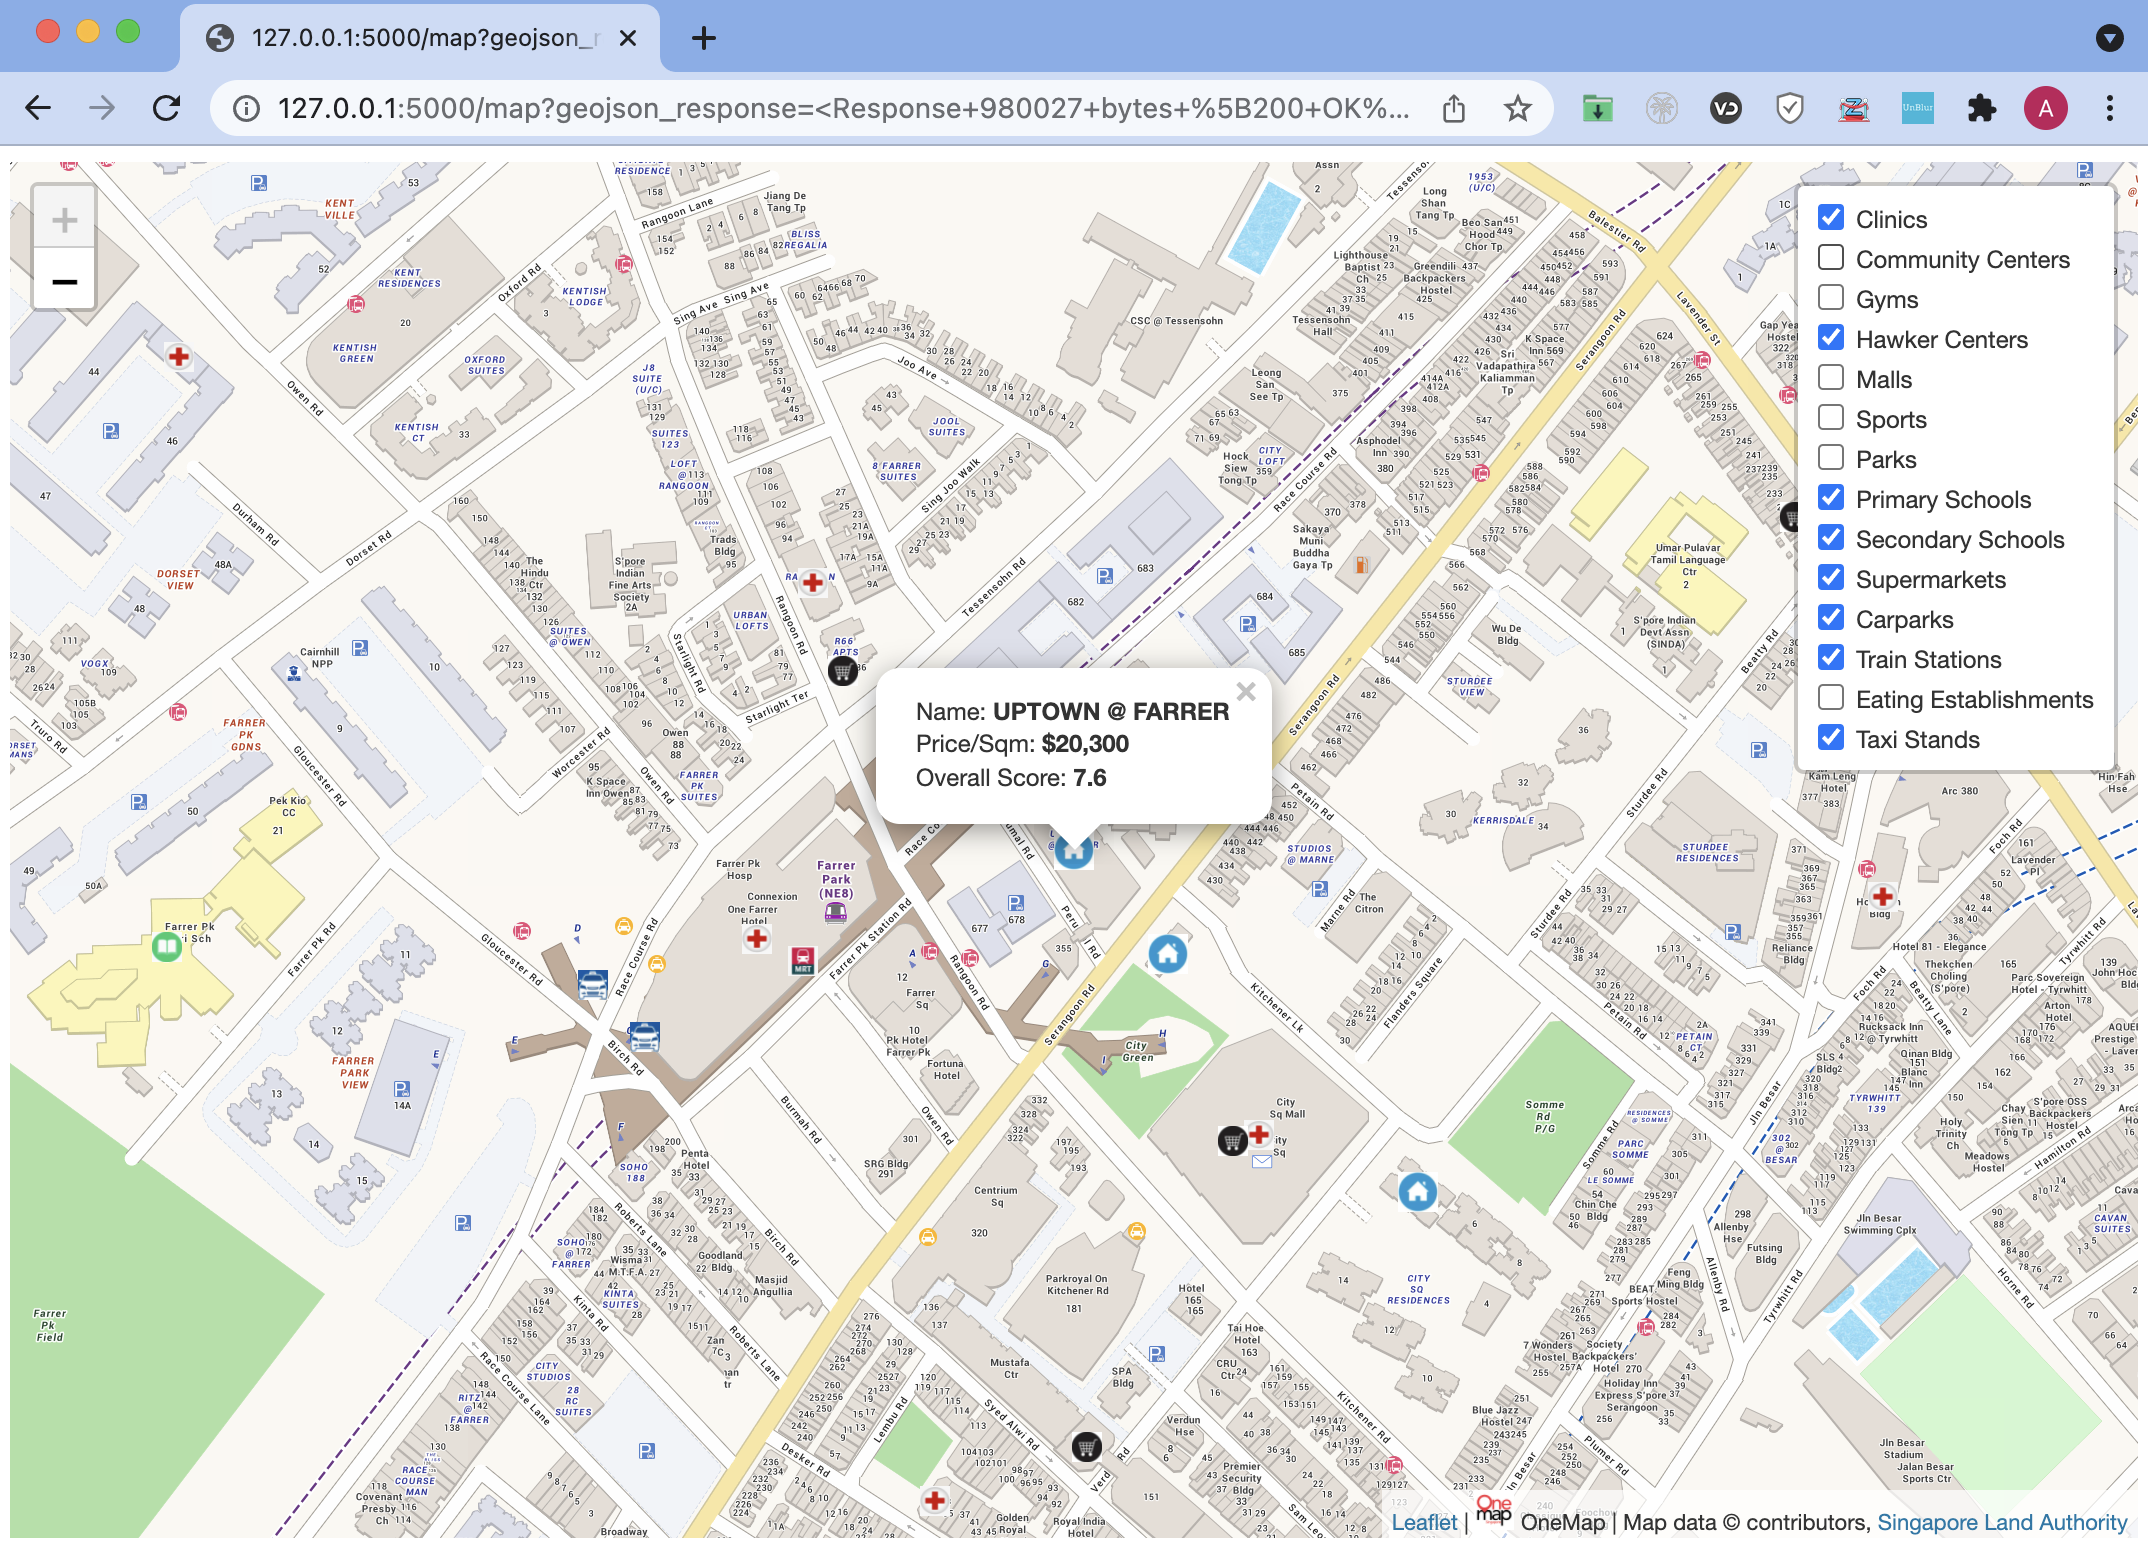
\includegraphics[width={0.5\textwidth}]{map.png}
   \caption{Example of a property recommendation and its neighboring amenities}
   \end{figure}
    
\section{Experiments}

\subsection{Experimental methodology}

Because our tool is meant to recommend homes according to the user-defined preferences, the key question is simply “are the recommended homes suitable for the user?”. We tested the effectiveness of our tool by evaluating the tool's recommendations for a few “personas” (user profiles) with constraints and preferences based on market research and our domain knowledge.

\subsection{Experimental results}

Tables 1 through 3 show the personas tested as well as the results. For each persona, we expected that the property projects recommended by the tool will only include those meeting the hard constraints defined, and that the neighborhood amenities will have high scores mostly in the top quartile. For each persona, the tool was configured with maximal weighting (100\%) for the preferred features and a small weightage (20\%) for the non-preferred features. Applying common sense and domain knowledge, we assessed the tool's recommendations for accuracy and relevancy. We also evaluated the tool's performance in terms of efficiency. The time between questionnaire submission and result visualization (corresponding to on-the-fly data retrieval, scoring, and recommendation) consistently took $<2$ seconds, providing a smooth user experience with minimal delay.

\begin{table}[ht]
    \centering
    \begin{tabular}{p{0.2\linewidth} | p{0.3\linewidth} | p{0.4\linewidth}} \hline
      & \textbf{Input parameters}  & \textbf{Results} \\ \hline
      \textbf{Constraints}& $<$\$5000/sqm, public housing, districts 27 \& 28
  & Compiled with hard constraints. \\ \hline
\textbf{Preferences} & Quality and quantity scores for primary and secondary schools, clinics, hawker centers. Quantity scores for subway (MRT) stations. & 7 out of the 9 quantity and quality scores for the preferred features were in the top quartile (Q4). The remaining two were within the second quartile (Q2). \\\hline
    \end{tabular}
    \caption{Persona 1: young parents with below-average income}
    \label{tab:my_label}
\end{table}

\begin{table}[ht]
    \centering
    \begin{tabular}{p{0.2\linewidth} | p{0.3\linewidth} | p{0.4\linewidth}} \hline
      & \textbf{Input parameters}  & \textbf{Results} \\ \hline
      \textbf{Constraints}& $<$\$8000/sqm, public or private housing, any district & Complied with hard constraints. \\ \hline
\textbf{Preferences} & 
Quantity and quality scores for sports facilities, gyms, community centers, parks, hawker centres. Quantity scores for F\&B, subway (MRT) stations, taxi stands. & 
10 out of the 13 quantity and quality scores for the preferred features were in the top quartile. The remaining three ranged between the 2nd and 3rd quartiles.

 \\\hline
    \end{tabular}
    \caption{Persona 2: single young adult with average income}
    \label{tab:my_label}
\end{table}


\begin{table}[ht]
    \centering
    \begin{tabular}{p{0.2\linewidth} | p{0.3\linewidth} | p{0.4\linewidth}} \hline
      & \textbf{Input parameters}  & \textbf{Results} \\ \hline
      \textbf{Constraints}& Between \$20,000 and \$30,000/sqm. Condominiums. Districts 9, 10, 11.
 & Complied with hard constraints. \\ \hline
\textbf{Preferences} & 
Quantity and quality scores for primary and secondary schools. clinics, sports facilities, gyms, community centers, parks, and malls. & The stricter constraints narrowed the shortlist to only 205 properties.
9 out of the 16 quantity and quality scores for the preferred features were in the top quartile. The remaining 7 ranged between the 2nd and 4th quartiles. 

 \\\hline
    \end{tabular}
    \caption{Persona 3: large multi-generational family, wealthy.
}
    \label{tab:my_label}
\end{table}


\section{Discussion}

In the first iteration of the tool, we had binned the quantity scores of the various attributes into quartiles. However, the results were not ideal, as the distribution of certain attributes (e.g. number of malls in the area) tended to fall within a fairly small range. As a result, the “top quartile” thresholds tended to be close to the median value. Instead of using quartiles, we changed our methodology. We first plotted out the distributions of all 15 attributes, and assigned attribute-specific bins of non-uniform widths to each attribute based on visual inspection and domain knowledge. For instance, the number of primary schools within the vicinity of a home was largely 2, causing the 25th and 50th percentile thresholds to both fall at 2. Applying our new methodology, having 1 school in the vicinity would result in a score of 0.25, 2 schools will score 0.5, 3 schools will score 0.75, and $>4$ schools will score 1.0. With this change in methodology, the top results tended to stand out more than the average housing project, providing better granularity and a more specific approach to scoring.

Similarly, for quality scores, we initially binned them into quartiles. However, since the median weighted ratings of amenities for a given housing project tended to be very close to one another, this resulted in very similar values in each of the bins. To remedy this, we applied min-max scaling instead, which allowed housing projects with high median weighted ratings of amenities to stand out more.

We are satisfied with the performance of the tool, as it helps to identify housing projects in ideal areas in an objective way and the interface is simple and intuitive. Even if the housing projects do not meet the user’s specific requirements, the suggestions indicate the appeal of the suggested areas and zones, and the user can thus focus their search on properties in these areas. 

The performance of the tool is not without limitations. We noted that the recommendations were often spatially clustered. This is expected since nearby housing projects have similar amenities. Further development may be done to enhance the tool, perhaps by including a heatmap of properties and scores, instead of simply showing the top 5 results. Furthermore, the information in the open-source databases we used was limited: for example, there was little info about the age of the housing projects. Because older homes tend to fetch a lower price, omission of age a configurable search parameter could lead to overrepresentation of these homes.

	\begin{thebibliography}{00} \footnotesize
		\bibitem{BengHuatChua}
		Beng Huat Chua (2015). \textit{Financialising Public Housing as an Asset for Retirement in Singapore}, International Journal of Housing Policy, 15:1, 27-42.
		\bibitem{CYYiu} C. Y. Yiu\& C. M. Hui (2005). \textit{An Empirical Study of the Impact of Income Uncertainty on Private Residential Property Markets in Singapore and Hong Kong}, Housing Studies, 20:5, 753-769.
		\bibitem{TeckChin} Teck Chin\& Geofrey Mills (1999). \textit{An Optimal Control Approach to Market Timing in the Singapore Property Market}, Journal of Real Estate Portfolio Management, 5:1, 83-94.
		\bibitem{Kavey} Kavey, Lee (1989). \textit{Condominium Search and Purchase Process}. Research Thesis. National University of Singapore, Singapore. Accessed at scholarbank.nus.edu.sg/handle/10635/163970.
		\bibitem{BangweonSong} Bangweon Song\& Seokjoong Kang (2015). \textit{A Method of Assigning Weights Using a Ranking and Nonhierarchy Comparison}, Advances in Decision Sciences, 2090-3359
		\bibitem{Morita} Morita, Masahiro\& Shinoda, Yoichi. (1994). \textit{Information Filtering Based on User Behavior Analysis and Best Match Text Retrieval}. 272-281. 10.1007/978-1-4471-2099-5\_28.
		\bibitem{Opricovic} Opricovic, Serafim\& Tzeng, Gwo-Hshiung. (2004). \textit{Compromise solution by MCDM methods: a comparative analysis of VIKOR and TOPSIS}, European Journal of Operational Research. 156. 445-455. 10.1016/S0377-2217(03)00020-1. 
		\bibitem{Isinkaye} Isinkaye, F. O., Folajimi, Y. O.,\& Ojokoh, B. A. (2015). \textit{Recommendation systems: Principles, methods and evaluation}, Egyptian Informatics Journal, 16(3), 261-273.
		\bibitem{Deldjoo} Deldjoo, Y., Dacrema, M.F., Constantin, M.G. et al. (2019). \textit{Movie genome: alleviating new item cold start in movie recommendation}, User Model User-Adap Inter 29, 291-343.
		\bibitem{Lops} Lops, P., Jannach, D., Musto, C. et al. (2019). \textit{Trends in content-based recommendation}, User Model User-Adap Inter 29, 239-249.
		\bibitem{Leskovec} Jure Leskovec, Anand Rajaraman, and Jeffrey David Ullman. (2014). \textit{Mining of Massive Datasets (2nd. ed.)}, Cambridge University Press, USA.
		\bibitem{Yang} Yang, J., et al. (2021). \textit{The financial impact of street-level greenery on New York commercial buildings.} Landscape and Urban Planning, 214, 104162.

	\end{thebibliography}
\end{document}